\documentclass[10pt,conference,compsocconf]{IEEEtran}

\usepackage{hyperref}
\usepackage{graphicx}	% For figure environment
\usepackage{array}
\usepackage{diagbox}
\usepackage{amssymb}
\usepackage{amsmath}
\usepackage[right=1cm,left=1cm,top=2cm,bottom=2cm]{geometry}
\begin{document}
\title{Machine learning - Project 1 report}
\author{Group 21 -- \textit{Volodymyr Loyko, Shiyue Nie, Thomas Sanchez}}

\maketitle

\section{Introduction}
This report will present the way we approached the problem of the classification of the Higgs Boson. We will first go through the transformation that we applied to the data, then move to the different methods we used to try to solve the problem and finally will speak in greater detail about our best submission.
\section{Formatting the Data}
The data we were given about the Higgs Boson contains 30 columns of measurements. Many of those columns contain NaNs, so it is needed to clean them before using them to predict the outcome of the experience on other data, in order to get unbiased results, as those NaNs, taking either the values $-999$ or $0$, are strong outliers. We will briefly describe all the techniques we used in order to format our data.

\textbf{1. Counting the NaNs :} First of all, we know that we will eventually get rid of the NaN values in our data, and we want to keep the information that they represent. Maybe having a NaN in a given column is correlated to the measurement of a Higgs Boson. What we did is add a column to our data which kept track of the number of NaN found in each row.

\textbf{2. Sanitation of the Data :} Now that the information about the NaN is stored in our data, we can safely remove them. We did the following for each column of our data which contained some invalid data. We first retrieved all the "valid" points in the column, i.e. those who did not have a NaN value, and then replaced the value of the unavailable points with the median of the valid points.  Note that we used the median and not the mean because the median is robust to outliers. Indeed, imagine we had all the points in the region $-1$ to $1$,the NaNs to $-999$ and an outlier at a very large value, then taking the average of the valid data including this large outlier would largely influence the result, while taking the median would ignore this outlier. 

\textbf{3. Standardization of the Data :} The second step in the formatting of our data was to standardize them. Having the gradient with the same magnitude in each direction yields a much faster convergence for the methods using gradient descent, like logistic regression. And it also turns out to be practical if we wish to construct a polynomial basis, as it will keep the large values of our data set bounded. It is important to note that in the case where a column has standard deviation $0$, i.e. all it values are the same, we then remove it from the data, as it contains no useful information.

\textbf{4. Polynomial basis :} The last step in the formatting of our data was to take a polynomial basis of degree $D$ for our data. We did not add the cross terms of the form $x_1x_2x_3$ for polynomials of degree three, as this would have given far too much features for our model to fit. For a basis of degree $D$, our polynomial basis was of the form
\begin{equation}
\left[1 ~ \mathbf{x}_1 \cdots \mathbf{x}_N ~\mathbf{x}_1^2 \cdots \mathbf{x}_N^2 ~ \mathbf{x}_1^D \cdots \mathbf{x}_N^D \right]
\end{equation}
where $\mathbf{x}_i \in \mathbb{R}^M, ~~i =1,\ldots,N$. 

\textbf{5. Additional notice :} When we turn to prediction, we will apply the same transformation to our testing set, but we will not recompute the median, mean and standard deviation, we will apply those that we had found for the training set, because we would otherwise end up with a biased result.
\section{Results}
\subsection{Methodology}
The methodology we followed to obtain our results was an extensive use of the cross validation while varying all the other parameters ($\lambda$ in the ridge regression as well as the polynomial degree) we had in a grid-search fashion. We would then choose the combination that yielded the minimal error, i.e. the smallest percentage of classification error. We did not iterate on $\gamma$ for the iterative methods, as the $\gamma$ will only change the speed of convergence of the method. We rather tried to pick on that seemed to work well and extended the number of maximal iterations, until convergence. 

\subsection{General results and comments}
Let us now present quickly some results that we obtained with each method. Note that, as the Ridge Regression stood quickly out as the best for our purpose, we did not extensively try to use the other methods, hence the results shown here for all other methods could easily be improved, and they are just present here for comparison's sake.
\begin{table}[!h]
	\centering
	\begin{tabular}{c||c|c|c|c|c|c}
		\textbf{Method used} & GD & SGD & LS & RR & LR & RLR  \\
		\hline
		\textbf{Accuracy ($\%$)} & $70.0$&$0$&$71.9$&$82.96$&$77.4$&$0.69$\\
		\hline
		\textbf{Degree} & $1$ &0&$1$&$10-14$&$2$&$3$\\
		\hline
		$\mathbf{\gamma}$ & $2^{-6}$&0&\diagbox{}&\diagbox{}&$10^{-8}$&$10^{-6}$\\
		\hline
		\textbf{max\_iters} & $2000$&0&\diagbox{}&\diagbox{}&$2000$&$2000$\\
		\hline
		$\mathbf{\lambda}$ & \diagbox{}&\diagbox{}&\diagbox{}&$0.7-54$&\diagbox{}&$7.74$\\
		
	\end{tabular}
	
	\caption{Best error in the measurements for respectively GD (Gradient Descent), SGD (Stochastic Gradient Descent), LS (Least Squares), RR (Ridge Regression), LR (Logistic Regression), RLR (Regularized Logistic Regression). The degree field corresponds to the degree of the polynomial basis we used for the prediction, the $\gamma$ is the parameter for every method implying some kind of gradient descent, max\_iters, $\lambda$ is the parameter for every method that implied penalization of the large weights. Note that the results for Ridge Regression seem quite vague, and it is because they were performed on a differently modified dataset. They will be given expensively in the table \ref{tab:RR}}
	\label{tab:results}
\end{table}

First of all, let us talk about our biggest surprise in the results. We would have expected both Logistic Regression (LR) and Regularized Logistic Regression (RLR) to do extremely well in this problem, as this is actually a classification problem : we must find whether the output is a Boson. However, we were not able to get very successful results with them, due to the fact that the convergence was very slow and that the picking of the parameter $\gamma$ was quite complicated.  Indeed, choosing it too large would cause the cost function to oscillate after a few hundreds of iterations, and picking it too small would cause the convergence to take tens of thousands of iterations. We did not try to dynamically adapt it, rather focusing on getting better results using the Ridge Regression. This convergence was slow even when trying to start with initial weights that were the result of a previous iteration with another method (e.g. the best $w$ from Ridge Regression, ...). Another problem linked to the fact that those methods are very slow is that they make cross-validation extremely painful, as the algorithm must compute thousands of slow steps for each method each time. However, we believe that if we had a more time and a deeper understanding of Regularized Logistic Regression, we could have got very good results with it, as it seems instinctively to be the most suited method for this problem : it is a classification method which allows for high degree polynomial basis, which allows to fit very non linear behaviors while not overfitting the data. 

We did not use the Gradient Descent and Stochastic Gradient descent very much, as they did not in this case present any advantage over the Least Squares and the Ridge Regression : they are iterative, depending on $\gamma$, while in the least squares, we only solve a linear system of equations. However, they are slightly faster than the logistic regression methods, as they do not require the evaluation of an exponential for each entry at each iteration. Another reason for not using it was that they tend to overfit the data if we start considering high degree polynomial basis as we typically did, as they do not penalize large weights.

The Least Squares has the advantage of being quick to compute, and giving a good solution immediately (the results it gives are good even with the raw data !). Its only problem is that it also overfits the data for bases with large polynomial bases, as it does not penalize weights, like (stochastic) gradient descent and logistic regression.

\subsection{Best results : Ridge Regression}
\subsubsection{Special formatting of our data}
Due to lack of time, we did not test this additional formatting of data with the other models. We only selected the model that was doing best already, and it was the Ridge Regression. What we did is split the dataset into four distinct datasets, using the JET\_split attribute to do so, as it ranges from $0$ to $3$ with only integer entries. It appeared then that some columns were filled with NaNs, and we then discarded them from the concerned datasets. The number of features then varied from a split to the other. We then split the testing data in the same fashion, and perform the prediction on each split dataset, before merging all the results we get. We also allowed each of the split dataset to be cross-validated on different parameters, in order to find relatively quickly the best value for each of them.


\subsubsection{Details of the results}
The detail of the results we obtained is summarised in the table \ref{tab:RR} below. We see that the prediction error is overall higher than in what we have in the table \ref{tab:results}. This could be because we have a smaller dataset each time that we train on, and so the result is slightly less precise than when we simulatneously train on the whole dataset. Note that the splits vary a lot in the number of elements in them, and that the splits $0$ and $1$ have way less features than others : it is due to the fact that some columns end up being filled only with $NaNs$ and are hence excluded as they do not bring any information.

\begin{table}[!ht]
	\centering
	\begin{tabular}{c||c|c|c|c}
		&\textbf{Split 0} & \textbf{Split 1} & \textbf{Split 2}& \textbf{Split 3}\\
		\hline
		\textbf{Size of the split} & $99913$ & $77544$& $50379$ & $22164$\\
		\hline
		\textbf{Number of features} & $19$ & $23$ & $30$ & $30$ \\
		\hline
		\textbf{Cross Validation Error (\%)} & $19.5$&$24.2$&$20.6$&$20.5$\\
		\hline
		\textbf{Degree} & $10$ & $12$ & $14$ & $14$ \\
		\hline
		{$\mathbf{\lambda}$} & $0.695$ & $2.976$ & $54.556$ & $26.367$\\
	\end{tabular}
	\caption{Expanded results for the best submission with Ridge Regression on a split dataset. The results are the ones with obtained with a cross-validation with several polynomial degrees and $\lambda$ ranging from $10^{-2}$ to $10^{2}$}
	\label{tab:RR}
\end{table}

Having this split dataset allows us a lot more flexibility in picking the weights and matches together particles that have the same behavior, hence the fact that it is our best result. We want also to show an example of cross-validation, on the figure \ref{fig:cross-validation} below.

\begin{figure}[!ht]
	\centering
	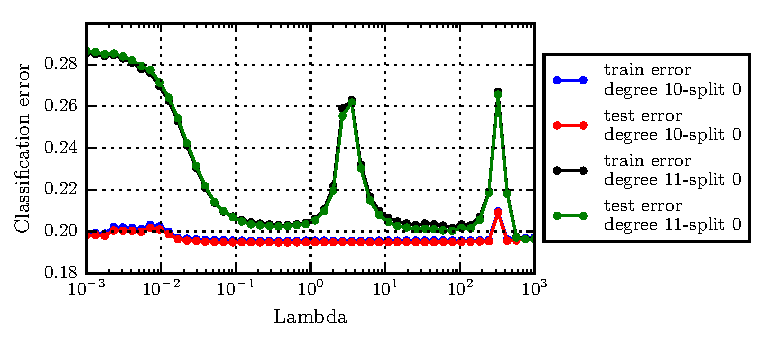
\includegraphics[scale=.7]{Cross_validation_10_11}
	\caption{Cross-Validation for the split $0$ for polynomials of degree $10$,$11$ and $\lambda$ ranging from $10^{-3}$ to $10^3$.}
	\label{fig:cross-validation}
\end{figure}

We have here in our figure a behaviour that could seem strange, because the cross-validation plot has peaks, and is flat otherwise. It is due to the fact we do not use a cost function here, but that we rather compute the classification error (in percentage of error). We know that a small cost function implies a small classification eror, but we also know that the converse is not true : a small classification error will not imply a small cost function. Hence, the graph that we have here can seem quite unpredictable. We choose to use the classification error over to usual cost function because it allowed for searching for a wider range of solutions : some that would not minimize the cost function, but would actually classify our data quite well.
\section{Conclusion}
We were able to approach the problem of finding the Higgs Boson from with quite different Machine Learning methods, but were very surprised in the result. While we expected the (Regularized) Logistic Regression to perform well, it presented too many fallbacks for us to use it reliably : the convergence was very slow, the result not extremely accurate. We used then the Ridge regression, which isn't iterative, and got our best results with it.
\end{document}
